% =====================================================================
%  POSTER A2 NGANG (594 x 420 mm). Bố cục theo mẫu poster HCMUTE (BM07A):
%  đầu poster, tóm tắt, I Đặt vấn đề, II Phương pháp, III Kết quả, IV Kết luận, tài liệu tham khảo.
%  Biên dịch: pdflatex -jobname="24119068_Huỳnh Lê Thành Nhân_Poster" vieedge_poster.tex
% =====================================================================
\documentclass{article}
\usepackage[T5]{fontenc}
\usepackage[utf8]{inputenc}
\usepackage[vietnamese]{babel}
\usepackage[scaled=.95]{helvet}
\renewcommand{\familydefault}{\sfdefault}
\usepackage[paperwidth=594mm,paperheight=420mm,margin=11mm]{geometry}
\usepackage{graphicx,booktabs,array,xcolor,enumitem,amsmath,amssymb,microtype}
\usepackage[many]{tcolorbox}
\usepackage{tikz}
\usepackage[hidelinks,pdftitle={VieEdge-Voice: Poster},pdfauthor={Huỳnh Lê Thành Nhân (24119068), Nguyễn Đoàn Hoàng Ngân (24119064)},unicode]{hyperref}
\usetikzlibrary{arrows.meta,positioning,calc}
% Thông tin chung cho bài báo và poster: sửa một chỗ ở đây.
\newcommand{\tenviet}{VieEdge-Voice: Trợ lý hỏi đáp bằng giọng nói tiếng Việt chạy hoàn toàn offline trên thiết bị biên}
\newcommand{\TENVIET}{VIEEDGE-VOICE: TRỢ LÝ HỎI ĐÁP BẰNG GIỌNG NÓI TIẾNG VIỆT CHẠY HOÀN TOÀN OFFLINE TRÊN THIẾT BỊ BIÊN}
\newcommand{\tenanh}{VieEdge-Voice: a fully offline Vietnamese voice question-answering assistant on edge devices}
\newcommand{\svmot}{Huỳnh Lê Thành Nhân}
\newcommand{\mssvmot}{24119068}
\newcommand{\svhai}{Nguyễn Đoàn Hoàng Ngân}
\newcommand{\mssvhai}{24119064}
\newcommand{\emailmot}{24119068@student.hcmute.edu.vn}
\newcommand{\truong}{Trường Đại học Công nghệ Kỹ thuật Thành phố Hồ Chí Minh}
\newcommand{\khoa}{Khoa Đào tạo tiên tiến}
\definecolor{xanhute}{HTML}{0272BC}
\definecolor{doute}{HTML}{D3202A}
\definecolor{dam}{HTML}{0B3C78}

\graphicspath{{../figures/}}
\pagestyle{empty}
\setlength{\parindent}{0pt}
\setlength{\parskip}{5pt}
\newcommand{\thanthan}{\fontsize{18.5}{23.5}\selectfont}
\setlist{itemsep=3pt,topsep=2pt,parsep=0pt,leftmargin=1em,label={\color{xanhute}$\blacksquare$}}
\newcommand{\phu}[1]{{\fontsize{22}{26}\selectfont\bfseries\color{dam}#1}\par\vspace{3pt}}
\newtcolorbox{cotk}[2]{enhanced,colback=white,colframe=white,boxrule=0pt,arc=0pt,left=0pt,right=0pt,top=0pt,bottom=0pt,
    width=#1,height=#2,nobeforeafter,box align=top,valign=top}
\newtcolorbox{cotp}[3]{enhanced,colback=white,colframe=white,boxrule=0pt,arc=0pt,left=0pt,right=0pt,top=0pt,bottom=0pt,
    width=#1,height=#2,nobeforeafter,box align=top,valign=top,before upper={\muc{#3}}}
\newcommand{\muc}[1]{{\fontsize{27}{31}\selectfont\bfseries\color{dam}#1}\par\vspace{-4pt}{\color{doute}\rule{42mm}{1.4mm}}\par\vspace{5pt}}
\newcommand{\so}[3]{% số lớn, nhãn, ghi chú
  \begin{tcolorbox}[enhanced,colback=dam!6,colframe=dam!6,boxrule=0pt,arc=2pt,left=6pt,right=4pt,top=5pt,bottom=4pt,width=\sow,height=41mm,nobeforeafter,box align=top,valign=top]
  {\fontsize{42}{46}\selectfont\bfseries\color{xanhute}#1}\par\vspace{1pt}
  {\fontsize{16.5}{20}\selectfont\bfseries #2}\par\vspace{0pt}
  {\fontsize{13.5}{16}\selectfont\color{black!70}#3}
  \end{tcolorbox}}
\newlength{\sow}\setlength{\sow}{64.5mm}
\newcommand{\hinh}[3]{\par\vspace{3pt}{\centering\includegraphics[width=#2]{#1}\par}\vspace{1pt}{\fontsize{15}{18}\selectfont\color{black!75}#3\par}\vspace{3pt}}

\begin{document}
\thanthan
\noindent\begin{minipage}[t][\textheight][t]{\textwidth}
% ---------------- ĐẦU POSTER ----------------
\noindent\begin{minipage}[c]{42mm}\centering
\includegraphics[height=44mm]{logo_truong.png}\end{minipage}\hfill
\begin{minipage}[c]{470mm}\centering
{\fontsize{41}{46}\selectfont\bfseries\color{dam}\TENVIET\par}
\vspace{5pt}
{\fontsize{24}{29}\selectfont\color{black!75}\tenanh\par}
\vspace{5pt}
{\fontsize{23}{28}\selectfont\textbf{\svmot} (MSSV \mssvmot) \quad \textbf{\svhai} (MSSV \mssvhai)\par}
\vspace{2pt}
{\fontsize{19}{23}\selectfont\khoa, \truong\ \ $\cdot$\ \ \emailmot\par}
\end{minipage}\hfill
\begin{minipage}[c]{46mm}\centering
\includegraphics[width=44mm]{logo_khoa_vuong.png}\end{minipage}

\vspace{6pt}{\color{xanhute}\rule{\textwidth}{1.2mm}}\par\vspace{6pt}
% ---------------- TÓM TẮT + CON SỐ CHÍNH ----------------
\noindent\begin{minipage}[t]{278mm}
{\fontsize{27}{31}\selectfont\bfseries\color{dam}TÓM TẮT}\par\vspace{2pt}
Trợ lý giọng nói phổ biến cần đám mây. VieEdge-Voice nghe, hiểu và trả lời bằng tiếng Việt hoàn toàn offline trên Raspberry Pi 5 (Yocto PREEMPT\_RT) và trong ứng dụng Android dùng NPU của Galaxy Z Fold7. Đề tài đo từng chặng của đường ống, chỉ ra thời gian đi đâu, giảm độ trễ có đối chứng, và so sánh trung thực các nền tảng, kể cả những gì không hiệu quả.
\end{minipage}\hfill
\begin{minipage}[t]{278mm}\vspace{2pt}
\so{1,53\,s}{Trả lời thật trên Fold7}{2 tỉ tham số, NPU, bật tra cứu, từ lúc nói xong}\hfill
\so{0,52\,s}{Câu có sẵn trên Pi}{đường nhanh, không qua LLM}\hfill
\so{0,041}{WER trên VIVOS}{Zipformer-vi, 300 câu}\hfill
\so{19-28\%}{Giảm đỉnh jitter}{Yocto-RT so với Pi OS, lõi âm thanh}
\end{minipage}

\vspace{7pt}
% ---------------- BỐN CỘT ----------------
\newlength{\cao}\setlength{\cao}{\dimexpr\textheight-127mm\relax}\newlength{\caoa}\setlength{\caoa}{.43\cao}\newlength{\caob}\setlength{\caob}{\dimexpr.57\cao-4pt\relax}
\newlength{\rong}\setlength{\rong}{138mm}
\noindent\begin{cotp}{\rong}{\cao}{I. ĐẶT VẤN ĐỀ}
Người nói giữ khoảng lặng rất ngắn giữa hai lượt lời [1], nên trợ lý được đánh giá bằng thời gian chờ. Đám mây giải quyết tốc độ, đổi lại cần mạng và phải đưa giọng nói ra khỏi thiết bị.

Trên thiết bị biên, mô hình phổ thông sai nhiều (Whisper-tiny sai 53\% số từ), đường ống nối tiếp cộng dồn độ trễ [2], Hailo-8L chỉ nhận mạng tĩnh.

\textbf{\color{dam}Mục tiêu:} trợ lý offline trọn vòng cho lúc mất sóng, như khi bão lũ, đo bằng cùng một quy ước trên máy nhúng và NPU điện thoại.

\textbf{\color{dam}Ưu điểm của thiết kế:}
\begin{itemize}
\item Xử lý hoàn toàn trên thiết bị: giọng nói không rời máy, chạy được khi mất mạng.
\item Một đường ống, chọn khối bằng cấu hình: chạy trên Pi 5 và trên điện thoại.
\item Đo từng chặng mỗi lượt: mọi tối ưu đều có số trước và sau.
\end{itemize}

\textbf{\color{dam}Tính năng:} hỏi đáp offline; 42 thẻ sơ cứu, thiên tai có nguồn; đường nhanh; tra cứu bật tắt; chạm để nói, ngắt lời; lọc ồn.

\textbf{\color{dam}Sản phẩm:} ứng dụng Android chạy trọn vòng; ảnh Yocto PREEMPT\_RT cho Pi 5; điện thoại làm micro, loa cho Pi; bảng điều khiển web.
\par\vspace{2pt}{\centering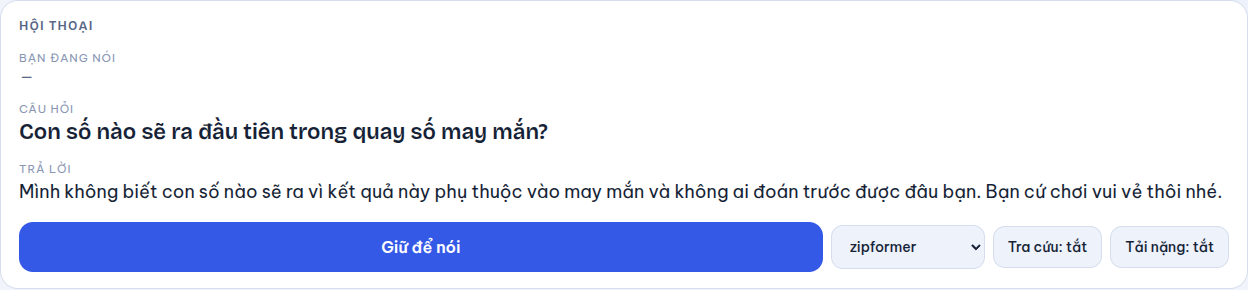
\includegraphics[width=\linewidth]{dashboard_hoithoai.png}\par}
{\fontsize{14}{17}\selectfont\color{black!75}\textbf{Hình.} Bảng điều khiển web (chạy minh hoạ trên máy tính xách tay).\par}
\end{cotp}\hspace{6mm}%
\begin{minipage}[t][\cao][t]{282mm}\vspace{2.1mm}
\begin{cotp}{282mm}{\caoa}{II. PHƯƠNG PHÁP}
{\centering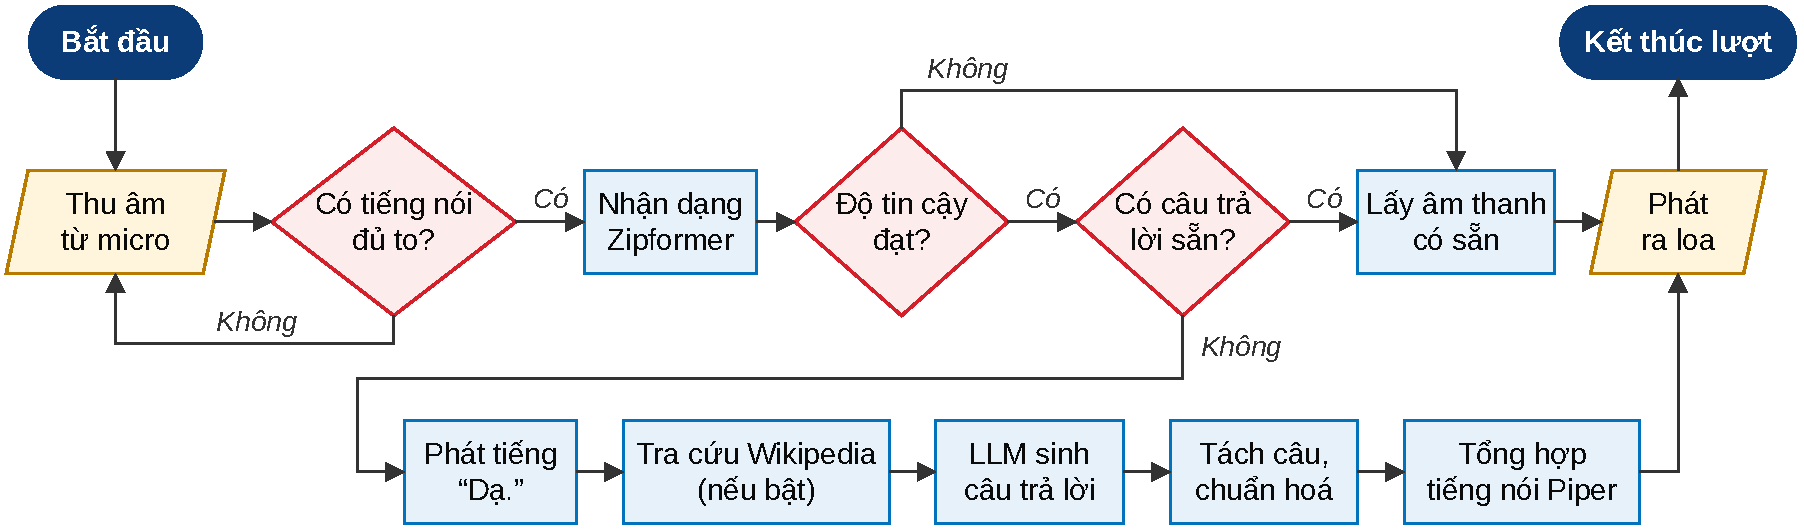
\includegraphics[width=232mm]{luu_do.pdf}\par}
\vspace{4pt}
{\fontsize{17.5}{22}\selectfont
\textbf{\color{dam}Giảm độ trễ:} đường nhanh bỏ qua tra cứu, LLM và TTS; cắt câu đầu sau 3 từ; xác nhận ``Dạ.'' chỉ giảm độ trễ cảm nhận. \textbf{\color{dam}Mô hình:} LoRA trên Qwen3.5 0,8 và 2 tỉ tham số; Q4\_0 cho dotprod nạp prompt nhanh hơn 43\%; STT Zipformer [3]; Pi dùng PREEMPT\_RT [4]. \textbf{\color{dam}Khác:} tra cứu 200.000 bài Wikipedia; lọc ồn RMS.\par}
\end{cotp}

\vspace{4pt}
\begin{cotp}{282mm}{\caob}{III. KẾT QUẢ}
\begin{minipage}[t]{136mm}
\hinh{latency.pdf}{136mm}{\textbf{Hình 1.} ``Dạ.'' kéo tiếng đầu xuống khoảng 0,5\,s; câu trả lời thật không sớm hơn. p50, 12 đến 13 lượt, giọng tổng hợp.}
\end{minipage}\hfill
\begin{minipage}[t]{136mm}
\hinh{stages.pdf}{94mm}{\textbf{Hình 2.} Cơ cấu thời gian; hai cấu hình khác nhau.}
\hinh{platform.pdf}{98mm}{\textbf{Hình 3.} NPU nạp prompt gấp 16 lần Pi, nên tra cứu chỉ thêm 0,06\,s (Pi: 1,4 đến 2,8\,s).}
\end{minipage}
\end{cotp}
\end{minipage}\hspace{6mm}%
\begin{cotk}{\rong}{\cao}
\vspace{4.2mm}\phu{Pi OS và Yocto-RT trên cùng Pi 5}
{\fontsize{16.5}{21}\selectfont\setlength{\tabcolsep}{4pt}\centering
\begin{tabular}{@{}l r r@{}}\toprule
Chỉ số & Pi OS & Yocto-RT\\\midrule
Jitter tải nặng 30 ph (µs) & 127 & \textbf{92}\\
Trả lời, yên, p50 (s) & 1,60 & 2,02\\
RAM sau khởi động (MB) & 442-538 & \textbf{285}\\
Công suất PMIC, yên (W) & 3,03 & \textbf{2,78}\\\bottomrule
\end{tabular}\par}
\vspace{3pt}
{\fontsize{16.5}{20}\selectfont So cặp 16 câu: chênh 0,06\,s, $p=0{,}40$. Không khẳng định được hệ nào nhanh hơn. Yocto-RT cho sự cô lập, không cho tốc độ suy luận.\par}
\hinh{jitter.pdf}{94mm}{\textbf{Hình 4.} Đuôi jitter 30 phút, 1,8 triệu mẫu.}
\phu{Nhiệt và công suất trên Fold7}
{\fontsize{16.5}{20}\selectfont 7,5 phút, 62 lượt: NPU tối đa 65\,°C, giữ 25,3 token/s. Cả máy 2,2 đến 3,3\,W.\par}
\vspace{5pt}
\muc{IV. KẾT LUẬN}
{\fontsize{17.5}{21.5}\selectfont
\begin{itemize}[itemsep=2pt]
\item Đạt chỉ tiêu tiếng đầu p95 dưới 1,5\,s (Pi 1,15\,s; Fold7 1,24\,s), 0 xrun, hoàn toàn offline.
\item Câu khẩn cấp trả lời bằng thẻ có nguồn: đúng thẻ 79/84 câu độc lập, không để LLM tự sinh lời khuyên.
\item Chưa đạt: encoder Hailo-8L lượng tử lệch (cosine 0,84, ngưỡng 0,9).
\item Hạn chế: giọng tổng hợp, 12 đến 16 lượt. Bước tiếp theo: đo với giọng người.
\end{itemize}\par}
\vspace{3pt}
{\fontsize{12.5}{15}\selectfont\color{black!75}\textbf{Tài liệu tham khảo.} [1] T. Stivers et al., PNAS 106(26), 2009. [2] T. Likhomanenko et al., ChipChat, arXiv:2509.00078, 2025. [3] Z. Yao et al., Zipformer, ICLR 2024. [4] F. Reghenzani et al., ACM CSUR 52(1), 2019.\par}
\end{cotk}
\end{minipage}
\end{document}
